\newpage
\chapter{Experiments and results}
\label{sec:experiments}

Prior to jumping to the final results obtained with our algorithm, this
chapter will attempt to give insight into the experiments we designed to verify our hypothesis. We examine our proposed methodology on two different but related scenarios. In the former scenario, we tackle the learning to count even hand-written digits, for the latter one, crowd counting problem is considered.   
This chapter contains experiments details, obtained results, comparison to similar works and finally a conclusion about the performance of our models in each of the experiments.

\section{Learning to count Even-odd hand-written digits}

We intend to explore the features learned when training a deep CNN, in order to understand their underlying representations. To this end, we designed a synthetic problem of counting even digits in images. This experiment clearly illustrates the basic idea behind this work, where we hypothesize that the features learned during this task are:
\begin{enumerate}
\item Efficient descriptors of digits to enable the model to count them.
\item Sufficiently representative of the digits to be applied for digits recognition tasks. 
\end{enumerate}

In this experiment, we feed images of digits into a deep convolutional neural network. Images are labeled with the number of even digits in each image. We apply a regression strategy to tackle this problem. Therefore, the output of the network is a single number determining the model's prediction for the amount of even digits present in the images. 
 

\subsection{Dataset} 
As it was meticulously described in (section ~\ref{subsubsec:digit}), we synthetically generated \textit{Even-odd digits dataset} to use for this task. the dataset holds the following properties:
\begin{itemize}
\item Images of MNIST hand-written digits where each image contains up to 15 digits. Also the images are made in gray-scale.
\item Each image has a dimension of $100\times100$. And each digit in the image is $18\times18$ pixels.  
\item A minimum distance of 18 pixels is considered between each two digits (from center to center) in an image to prevent overlapping.
\item The dataset is generated uniformly. It means that there are equal number of images for each amount of digits in the image. For instance, the number of images with 5 even digits are the same as number of images containing 10 even digits.
\item The dataset of 1,000,000 samples is divided into a training set of 800,000 and a test set of 200,000. 
\end{itemize}

Since we use Caffe platform to do our experiments, we convert the images into LMDB format. LMDB uses memory-mapped files, so it has the read performance of a pure in-memory database while still offering the persistence of standard disk-based databases, and is only limited to the size of the virtual address space, (it is not limited to the size of physical RAM). Therefore, we created two LMDB files for training and testing sets to be fed to the network.  

\subsection{Learning process}

As discussed in chapter~\ref{subsubsec:digitarch}, for learning to count the number of even digits, we designed a deep CNN. Table~\ref{fig:digitnet} shows a review of the network's specification and architecture.

\begin{table}[H]
	\centering
			\caption{The deep CNN with 2 convolution layers to count the number of even digits.}
	\begin{tabular}{ |p{2cm}|p{2cm}| }
	\hline 
	\multicolumn{2}{|c|}{\textbf{Network parameters}} \\
	\hline
	\hline
	\textbf{Layers} & \textbf{setting }\\
	\hline
	Conv1 & $20\times15\times15$\\
	\hline
	ReLU1 & max(x,0)  \\
	\hline
	LRN1 & $\alpha$=0.0001, $\beta$=0.75\\
	\hline
	Pool1    & $max(2\times2)$ \\
	\hline
	Conv2 & $50\times3\times3$\\
	\hline
	ReLU2 & max(x,0)  \\
	\hline
	LRN2 & $\alpha$=0.0001, $\beta$=0.75\\
	\hline
	Pool2    & $max(2\times2)$ \\
	\hline
	IP1 & 64 outputs \\
	\hline
	ReLU3 & max(x,0)  \\
	\hline
	IP2 & 1 outputs \\
	\hline
	\end{tabular}
		\label{fig:digitnet}
\end{table}




However, a well-designed network solely cannot guarantee an optimal performance for the model. The responsibilities of learning are divided between the Net for yielding loss and gradients, and the optimization methods and parameters for overseeing the optimization and generating parameter updates. 

Among Caffe solvers, As described in section~\ref{subsec:sgd}, we use Stochastic Gradient Descent optimization method. Apart from solver method, we solver parameters need to be set attentively in order to optimize the model performance. Table~\ref{tab:digitsolver} summarizes the initial settings for the solver parameters while the upcoming items justify our decisions.

\begin{table}[H]
	\centering
			\caption{The solver parameters settings for even digit counting problem.}
	\begin{tabular}{ |p{2cm}|p{2cm}| }
	\hline 
	\multicolumn{2}{|c|}{\textbf{Optimization parameters}} \\
	\hline
	\hline
	\textbf{Parameter} & \textbf{value}\\
	\hline
	base\_lr & 0.0001\\
	\hline
	batch size & 256\\
	\hline
	momentum & 0.9  \\
	\hline
	weight decay & 0.0005\\
	\hline
	step size   & 40000 \\
	\hline
	gamma($\gamma$) & 0.1\\
	\hline
	iterations & 1,600,000\\
	\hline
	\end{tabular}

		\label{tab:digitsolver}
\end{table}


\begin{itemize}
\item \textbf{Learning rate:} The basic learning rate is 0.0001. However, for our experiment we chose \textit{multi-step} learning policy in which, after each \textit{stepsize}=40000 iterations, the learning rate drops by the rate of $\gamma = 0.1$. This initialization is based on rules of thumbs used in \cite{krizhevsky2012imagenet}.
\item \textbf{Batch size:} Due to the non-complex and low-resolution dataset we are training on, we were able to use batches of size 256 for our training and testing phases.
\item \textbf{Momentum:} We use momentum $\mu = 0.9$. This selection also is based one rules of thumbs. Because, momentum setting $\mu$ effectively multiplies the size of our updates by a factor of $\frac{1}{1-\mu}$. Hence, changes in momentum and learning rate ought to be accompanied with an inverse correlation. When momentum $\mu = 0.9$, we have an effective update size of 10 since we also drop the learning rate by the factor of $\gamma= 0.1$.
\item \textbf{Weight decay:} Weight decay as a penalty term to the error function, has a constant value of 0.0005. This decay constant is multiplied to the sum of squared weights.
\item \textbf{Iterations:} Given the time and hardware we had, we managed to let the system train for 1,600,000 iterations
\end{itemize}

\noindent The algorithm trained on a GPU NVIDIA \cite{kirk2007nvidia} Tesla K40 \cite{lindholm2008nvidia}.It took almost 4 days to train 800,000 samples and tested over 200,000 images. The learning curves of this learning process are shown in the figure~\ref{fig:curve}

\begin{figure}[H]
	\centering
	{
\includegraphics[width=0.7\textwidth]{images/1}}
	\caption{}
	\label{fig:curve}
\end{figure}

\textbf{ADD EXPLANATION OF THE LEARNING CURVES}

\noindent Moreover, figure~\ref{fig:feat} illustrates the features learned from one input sample at each convolutional layer in the network.


\begin{figure}[H]
	\centering
	{
\includegraphics[width=0.7\textwidth]{images/1}}
	\caption{}
	\label{fig:feat}
\end{figure}

\textbf{ADD EXPLANATION OF THE FEATURES}
 
%Moreover, a schematic of the model with the output of each layer is depicted in figure~\ref{fig:digitnet}.
%%\begin{figure}[H]
%%	\centering
%	{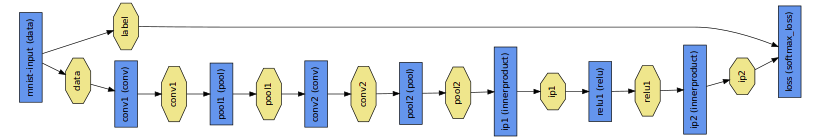
\includegraphics[width=1\textwidth]{images/caffe}}
%	\caption{An MNIST digit classification example of a Caffe network, where blue boxes represent layers and yellow octagons represent data blobs produced by or fed into the layers\cite{jia2014caffe}.}
%	\label{fig:digitnet}
%\end{figure}
\textbf{A SHORT TRANSITIVE PARAGRAPH TO GO TO RESULTS}

\subsection{Results}

In addition to the Euclidean loss function we implemented in our architecture, we use two other error measurements to evaluate and compare the performance of our model. These measurements are briefly described and justified in below:
\begin{enumerate}
\item \textbf{Mean squared error(MSE)}: Mean squared error is arguably the most important criterion used to evaluate the performance of a predictor or an estimator. The mean squared error is also useful to relay the concepts of bias, precision, and accuracy in statistical estimation. The MSE is the second moment (about the origin) of the error, and thus incorporates both the variance of the estimator and its bias \cite{lehmann1998theory}. The MSE can be estimated by
$$MSE = {\frac{1} {N}{\sum\limits_{i = 1}^N {(\hat{x_{pred}} - x_{obs} } })^{2} } $$
where:\\
\textit{N}: the number of instances\\
\textit{ $\hat{x_{pred}}$}: a vector of N predictions\\
\textit{$x_{obs}$}: a vector of observed value (ground truth) for input x\\

The mathematical benefits of mean squared error are particularly evident in its use at analyzing the performance of linear regression, as it allows one to partition the variation in a dataset into variation explained by the model and variation explained by randomness.
\item \textbf{Mean absolute error(MAE)}: MAE measures the average magnitude of the errors in a set of predictions, without considering their direction. In other words, it measures how close predictions are to the eventual outcomes \cite{willmott2005advantages}. MAE can simply be computed by:
$$MAE = {\frac{1} {N}{\sum\limits_{i = 1}^N {|x_{pred} - x_{obs} } }| } $$
where:\\
\textit{N}: number of instances\\
\textit{ $x_{pred}$}: prediction for instance x\\
\textit{$x_{obs}$}: observed value (ground truth) for instance x
\end{enumerate}

\noindent Having our used error measurements explained, for the task of counting even digits, using 800,000 training samples and 200,000 test images, and after 1,600,000 iterations, our model obtained the following results:


\begin{table}[H]
\caption{Table caption font is different from the normal text font in order to get a better differentiation -- I like it that way.}
\centering
\small\sffamily
\begin{tabular}{llr}
%\toprule
\multicolumn{2}{c}{\textbf{\textbf{Results}}} \\
\bottomrule
\textbf{Error measurement}        & \textbf{Error} \\
\bottomrule
%\midrule
Euclidean loss           & 0.20  \\
Mean squared error       & 0.20  \\
Mean absolute error      & 0.20  \\
\bottomrule
\end{tabular}
\end{table} 

Accordingly, the spread-error plot corresponding to the model is provided.

\begin{figure}[H]
	\centering
	{
\includegraphics[width=0.7\textwidth]{images/1}}
	\caption{}
	\label{fig:splot}
\end{figure}

As you may observe in Figure~\ref{fig:splot}, most
of the frames are correctly labeled. Moreover, most of the
errors correspond to adjacent number values.

A similar experiment was done by \citeauthor*{segui2015learning}. In their work, they used images with up to 5 digits with slightly different architecture. Also each digit in the images had a dimension of $28\times28$. They approached the problem as a classification task. 

\indent Therefore, in order to provide a fair comparison, we demonstrate the difference the accuracy of both experiments from random, and from there we draw a proportional comparison. These comparison has been shown in the table~\ref{tab:comp}.

\begin{table}[H]
\caption{Table caption font is different from the normal text font in order to get a better differentiation -- I like it that way.}
\centering
\small\sffamily
\begin{tabular}{llr}
%\toprule
\multicolumn{3}{c}{\textbf{\textbf{Performance Comparison}}} \\
\bottomrule
\textbf{Experiments}  & \textbf{Chance} & \textbf{Accuracy} \\
\bottomrule
%\midrule
Euclidean loss           & 0.20 & 0.30 \\
Mean squared error       & 0.20 & 0.30 \\

\bottomrule
\end{tabular}
\end{table} 

\textbf{EXPLANATION OF THE COMPARISON}

\subsection{Conclusion}

\textbf{CONCLUSION AFTER THE EXPERIMENT} 

\section{Counting pedestrians in a walkway}

